
%(BEGIN_QUESTION)
% Copyright 2010, Tony R. Kuphaldt, released under the Creative Commons Attribution License (v 1.0)
% This means you may do almost anything with this work of mine, so long as you give me proper credit

In this circuit, an electronic differential pressure transmitter with a 4-20 mA output signal connects to a local pressure indicator and to a remote pressure indicator.  Your task is to figure out how to connect the loop calibrator to force the remote indicator (only) to register a pressure of 300 PSI, without interrupting or otherwise affecting the transmitter's signal to the local indicator:

$$\includegraphics[width=15.5cm]{i00627x01.eps}$$

Sketch your solution, showing both the loop calibrator's test lead connections and the mode it must be set to ({\it source}, {\it read}, or {\it simulate}).  Assume a transmitter calibration of $-10$ PSI to +440 PSI.

\vfil

Note: there is more than one correct answer to this question!

\underbar{file i00627}
\eject
%(END_QUESTION)





%(BEGIN_ANSWER)

This is a graded question -- no answers or hints given!

%(END_ANSWER)





%(BEGIN_NOTES)

First, we will need to figure out how to isolate the remote indicator from the rest of the circuit, so that the transmitter still receives loop power and the local indicator still registers the transmitter's signal.  One way to do this is to connect a temporary ``jumper wire'' bypassing the remote indicator, then disconnect one of the normal wires from a terminal on the remote indicator.

\vskip 10pt

Next, we will calculate the amount of current necessary from the loop calibrator in order to simulate a 300 PSI condition.  We know that the transmitter's range is $-10$ PSI to +440 PSI.  Therefore, a pressure of +300 PSI will be 310 PSI above the ``zero'' point over a span of 450 PSI, and therefore will represent a percentage of range equal to ${310 \over 450} = 68.66\%$.  Converting a 68.66\% signal into milliamps over a 4-20 mA range, we get {\bf 15.02 mA}.

\vskip 10pt

Solution using the loop calibrator to {\it source} current:

$$\includegraphics[width=15.5cm]{i00627x02.eps}$$


%INDEX% Electronics review: 4-20 mA loop calibrator (test equipment)

%(END_NOTES)


